\section{Rotation of a Rigid Body}

\subsection{Rotational Motion}

A \textbf{rigid body} is an extended object whose size and shape do not
change as it moves.  That is, it cannot be stretched, compressed, or
deformed.  All points on the body have the same angular velocity and
angular acceleration.

\begin{figure}
    \centering
    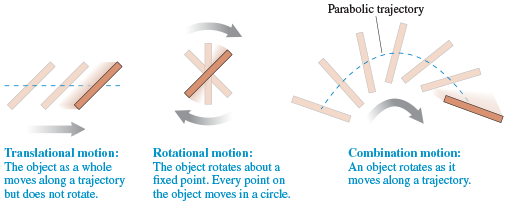
\includegraphics[width=0.4\textwidth]{../figures/basic-types-of-motion.png}
    \caption{Three basic types of motion of a rigid body.}%
    \label{fig:basic-types-of-motion}
\end{figure}

Figure~%
\ref{fig:basic-types-of-motion} shows three basic types of motion of a
rigid body:
\begin{itemize}
    \item
        Translational motion
    \item
        Rotational motion
    \item
        Combination motion
\end{itemize}

\subsection{Rotation About the Center of Mass}

\begin{figure}
    \centering
    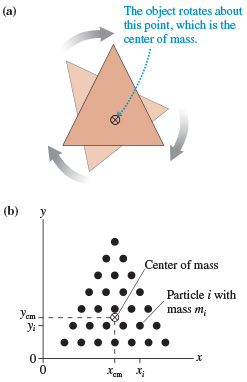
\includegraphics[width=0.4\textwidth]{../figures/rotation-center-of-mass.png}
    \caption{Rotation about the center of mass.}%
    \label{fig:rotation-center-of-mass}
\end{figure}

An unconstrained object (i.e., one not on an axle) on which there is no
net force rotates about a point called the \textbf{center of mass}.  The
center of mass remains motionless while every other point in the object
undergoes circular motion around it.

To locate the center of mass, Figure~%
\ref{fig:rotation-center-of-mass}b models the object as a set of
particles numbered
$
    i = 1, 2, 3, \dots
$%
.  Particle
$
    i
$ has mass
$
    m_i
$ and is located at position
$
    (x_i,y_i)
$%
.  The center of mass is located at position
\begin{align}
    x_\mathrm{cm} &= \frac{1}{M} \sum_i m_ix_i \\
    y_\mathrm{cm} &= \frac{1}{M} \sum_i m_iy_i
\end{align}
where
$
    M = m_1 + m_2 + m_3 + \dots
$ is the object's total mass.

\subsection{Rotational Energy}

A rotating rigid body has kinetic energy called rotational kinetic
energy.

\begin{figure}
    \centering
    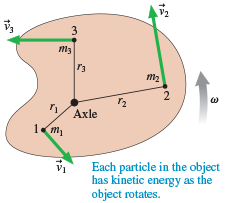
\includegraphics[width=0.4\textwidth]{../figures/rotational-kinetic-energy.png}
    \caption{Rotational kinetic energy is due to the motion of the
    particles}%
    \label{fig:rotational-kinetic-energy}
\end{figure}

Figure~%
\ref{fig:rotational-kinetic-energy} shows a few of the particles making
up a solid object that rotates with angular velocity
$
    \omega
$%
.  For each particle
$
    i
$ which rotates in a circle of radius
$
    r_i
$%
,
$
    i
$ moves with speed
$
    v_i = r_i\omega
$%
.  The object's rotational kinetic energy is the sum of the kinetic
energies of each of the particles
\begin{equation}
    K_\mathrm{rot} = \frac{1}{2}\left(\sum_i m_i r_i^2\right)\omega^2
\end{equation}
where the quantity
$
    \sum_i m_ir_i^2
$ is called the object's \textbf{moment of inertia
$
    I
$}:
\begin{equation}
    \label{eq:moment-of-intertia} I = \sum_i m_ir_i^2
\end{equation}
The units of
$
    I
$ are
$
    \unit{\kilo\gram\square\metre}
$%
.  An object's moment of inertia depends on the axis of rotation.  Once
the axis is specified, the values of
$
    r_i
$ can be determined.

Written using moment of inertia
$
    I
$%
, the rotational kinetic energy is
\begin{equation}
    \label{eq:rotational-kinetic-energy} K_\mathrm{rot} = \frac{1}{2}I\omega^2
\end{equation}

\begin{Exercise}[title={A rotating widget}]
    \begin{center}
        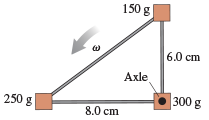
\includegraphics[totalheight=0.2\textheight]{../figures/rotating-widget.png}
        \captionof{figure}{The rotating widget.}%
        \label{fig:rotating-widget}
    \end{center}
    At what angular velocity does the widget, shown in Figure~%
    \ref{fig:rotating-widget}, have
    $
        \qty{100}{\milli\joule}
    $ of rotational energy.
\end{Exercise}
\begin{Answer}
    The moment of inertia is measured about the rotation axis, thus
    \begin{align}
        I &= \sum_i m_ir_i^2 = (\qty{.25}{\kilo\gram})(\qty{.080}{\metre}^2)
        + (\qty{.15}{\kilo\gram})(\qty{0.060}{\metre}^2) + (\qty{0.30}{\kilo\gram})
        (\qty{0}{\metre}^2) \\
        &= \qty{2.14e-3}{\kilo\gram\square\metre}
    \end{align}
    With
    $
        I
    $ known, solve for
    $
        \omega
    $ from Equation~%
    \ref{eq:rotational-kinetic-energy}.
\end{Answer}

Notice that
$
    moment of inertia is the rotational equivalent of mass
$%
.  It plays the same role in Equation~%
\ref{eq:rotational-kinetic-energy} as mass
$
    m
$ in
\begin{equation}
    K = \frac{1}{2}mv^2
\end{equation}
The quantity mass us the same as the measure of inertia.  Objects with
larger mass have a larger inertia, meaning that they're harder to
accelerate.  Similarly, an object with a larger moment of inertia is
harder to rotate.

For example, consider two wheels with the same total mass
$
    M
$ and radius
$
    R
$%
.  How the weight is distributed will determine the inertia of the
wheel.  A wheel with the weight closer to the axis of rotation is easier
to spin than the wheel with the mass distributed at the edge of it.

If the rotation axis is not through the center of mass, then rotation
may cause the center of mass to move up or down.  In that case, the
object's gravitation potential energy
\begin{equation}
    U_\mathrm{G} = Mgy_\mathrm{cm}
\end{equation}
will change.  If there are no dissipative forces and no work is done by
external forces, then the mechanical energy
\begin{equation}
    E_\mathrm{mech} = K_\mathrm{rot} + U_\mathrm{G}
\end{equation}
is a conserved quantity

\subsection{Calculating Moment of Inertia}

For an object where the points of masses are not clear, we need to think
carefully about each of of the terms in the Equation~%
\ref{eq:moment-of-intertia}.  The equation asks us to sum over each
``piece of mass'' a certain distance from the axis of rotation.  But
what exactly does each ``piece of mass'' mean?  It means we need to use
an infinitesimally small piece of mass shown in Figure~%
\ref{fig:infinitesimally-small-piece-of-mass}.

\begin{figure}
    \centering
    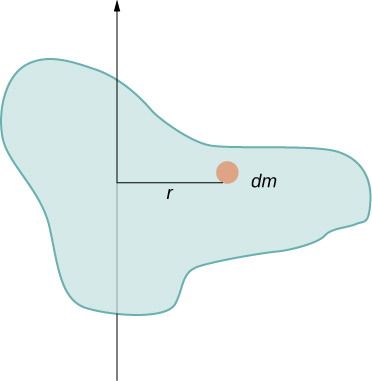
\includegraphics[width=0.4\textwidth]{../figures/infinitesimally-small-piece-of-mass.jpg}
    \caption{Using an infinitesimally small piece of mass to calculate
    contribution to the moment of inertia.}%
    \label{fig:infinitesimally-small-piece-of-mass}
\end{figure}

The need to us ean infinitesimally small piece of mass
$
    \dif m
$ suggests that we can write the moment of inertia by evaluating an
integral over infinitesimal masses rather than doing a discrete sum over
finite masses:
\begin{equation}
    I = \sum_i m_ir_i^2 = \int r^2 \dif m
\end{equation}

If a complex object can be divided into simpler pieces
$
    1, 2, 3, \dots
$ whose moments of inertia
$
    I_1, I_2, I_3, \dots
$ are already known, the moment of inertia of the entire object is
\begin{equation}
    I_\mathrm{object} = I_1 + I_2 + I_3 + \dots
\end{equation}

\subsubsection{The Parallel-Axis Theorem}

\begin{figure}
    \centering
    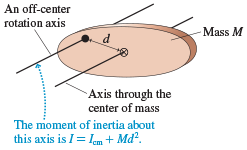
\includegraphics[width=0.4\textwidth]{../figures/an-off-center-axis.png}
    \caption{An off-center axis.}%
    \label{fig:an-off-center-axis}
\end{figure}

The moment of inertia depends on the rotation axis.  Suppose you need to
know the moment of inertia for rotation about the off-center axis in
Figure~%
\ref{fig:an-off-center-axis}.  You can find this quite easily if you
know the moment of inertia for rotation around a \emph{parallel axis}
through the center of mass.

If the axis of interest is distance
$
    d
$ from a parallel axis through the center of mass, the moment of inertia
is
\begin{equation}
    I = I_\mathrm{cm} + Md^2
\end{equation}

\subsection{Torque}

\begin{figure}
    \centering
    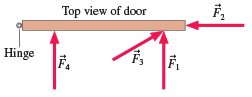
\includegraphics[width=0.4\textwidth]{../figures/four-forces-on-door.png}
    \caption{The four forces have different effects on the swinging
    door.}%
    \label{fig:four-forces-on-door}
\end{figure}

Consider the common experience of pushing open a door.  Figure~%
\ref{fig:four-forces-on-door} is a top view of a door hinged to the
left.  Four pushing forces are shown, all of equal strength.  Which of
these will be most effective at opening the door.

Force
$
    \vec{F}_1
$ will open the door, but force
$
    \vec{F}_2
$%
, which pushes straight at the hinge will not.  Force
$
    \vec{F}_3
$ will open the door, but not as easily as
$
    \vec{F}_1
$%
.  Force
$
    \vec{F}_4
$ is perpendicular to the door but pushing close to the hinge is not as
effective as pushing at the outer edge of the door.

The ability of a force to cause a rotation depends on three factors:
\begin{enumerate}
    \item
        The magnitude
        $
            F
        $ of the force.
    \item
        The distance
        $
            r
        $ from the point of the application to the pivot.
    \item
        The angle at which the force is applied.
\end{enumerate}

We can incorporate these three factors into a single quantity called the
\emph{torque}.
\begin{equation}
    \tau = r F\sin{\oslash}
\end{equation}

\begin{figure}
    \centering
    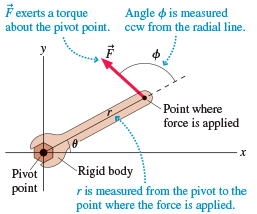
\includegraphics[width=0.4\textwidth]{../figures/torque-diagram.png}
    \caption{Force
    $
        \vec{F}
    $ exerts a torque about the pivot point.}%
    \label{fig:torque-diagram}
\end{figure}

Figure~%
\ref{fig:torque-diagram}shows a force
$
    \vec{F}
$ trying to rotate the wrench and nut about a \emph{pivot point}--the
axis about which the nut will rotate.  We say that this force exerts
\textbf{torque}
$
    \tau
$%
.  \textbf{Torque is the rotational equivalent of force}

Torque, like force, has a sign.  A torque that tries to rotate the
object in a ccw direction is positive while a negative torque gives a cw
rotation.  A force pushing straight toward the pivot or pulling straight
out from the pivot exerts no torque.

\subsubsection{Interpreting Torque}

Torque can be interpreted from two perspectives, as shown in Figure~%
\ref{fig:interpretations-of-torque}.  First, the quantity
$
    F\sin{\oslash}
$ is the tangential force component
$
    F_\mathrm{t}
$%
.  Consequently, the torque is
\begin{equation}
    \tau = rF_\mathrm{t}
\end{equation}

\begin{figure}
    \centering
    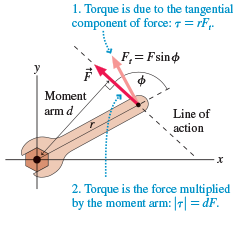
\includegraphics[width=0.4\textwidth]{../figures/interpretations-of-torque.png}
    \caption{Two useful interpretations of the torque}%
    \label{fig:interpretations-of-torque}
\end{figure}

I.e., torque is the product of
$
    r
$ with the force component
$
    F_\mathrm{t}
$ that is tangent to the circular path followed by this point on the
wrench.

A second perspective is based on the idea of a \emph{moment arm}.
Figure~%
\ref{fig:interpretations-of-torque} shows the \textbf{line of action},
the line along which the force acts.  The minimum distance between the
pivot point and the line of action is called the \textbf{moment arm}
$
    d
$%
.  Because
$
    \sin{\qty{180}{\degree} - \oplus} = \sin{\oplus}
$%
, it is easy to see that
$
    d=rsin\oplus
$%
.  Thus,
$
    \tau
$ can be rewritten as
\begin{equation}
    |\tau| = dF
\end{equation}

\subsection{What is the center of mass?}

The \emph{center of mass} is a position defined relative to an object or
system of objects.  It is the average position of all parts of the
system

For simple rigid objects with uniform density, the center of mass is
located at the \textbf{centroid}.  For complicated shapes, with
nonuniform density:  we need a more general mathematical definition of
the center of mass.

Imagine a rod with a negligible mass that has hanging weights
distributed across the rod with gravity being the only force acting upon
it, if you placed a pivot point at the C.O.M., the rod would not tip one
weight or another.  That is, for the rod to stay perfectly balanced the
net torque would have to be zero
\begin{equation}
    \tau_\mathrm{net} = 0
\end{equation}
For each weight
$
    i
$%
,
\begin{equation}
    \tau_\mathrm{net} = \sum_i \tau_i = m_1g(x_1-x_\mathrm{cm})+m_2g(x_2-x_\mathrm
    {cm})+m_3g(x_3-x_\mathrm{cm}) + \dots = 0
\end{equation}
We then solve for
$
    x_\mathrm{cm}
$
\begin{align}
    0 &= m_1g(x_1-x_\mathrm{cm})+m_2g(x_2-x_\mathrm{cm})+m_3g(x_3-x_\mathrm
    {cm}) + \dots \\
    &= m_1(x_1-x_\mathrm{cm})+m_2(x_2-x_\mathrm{cm})+m_3(x_3-x_\mathrm{cm})
    + \dots \\
    &= m_1x_1 + m_2x_2 + m_3x_3 + \dots - m_1x_\mathrm{cm} -m_2x_\mathrm
    {cm} - m_3x_\mathrm{cm} + \dots \\
    &= m_1x_1 + m_2x_2 + m_3x_3 + \dots - x_\mathrm{cm}(m_1 + m_2 + m_3
    + \dots) \\
    x_\mathrm{cm}(m_1 + m_2 + m_3 + \dots) &= m_1x_1 + m_2x_2 + m_3x_3 +
    \dots \\
    x_\mathrm{cm} &= \frac{m_1x_1 + m_2x_2 + m_3x_3 + \dots}{m_1 + m_2 +
    m_3 + \dots}
\end{align}

\subsubsection{What is useful about the center of mass?}

The unique property of the C.O.M.  of an object or an system is that it
is the point where any uniform force on the object acts.

For the purposes of calculation, we can treat any oddly-shaped object as
if all its mass is concentrated in a tiny object located at the center
of mass.  Additionally, if you apply a force at the center of mass it
will not spin and only translate.

\subsection{Rotational Dynamics}

A torque causes an angular acceleration, like how force causes an
acceleration.

\begin{equation}
    \alpha = \frac{T_\mathrm{net}}{I}
\end{equation}

\subsubsection{Problem Solving Strategies}

Model the object as a rigid body

\begin{itemize}
    \item
        Identify the axis about which the object rotates
    \item
        Identify the forces and determine their distances from the axis
    \item
        Identify any torques caused by the forces and the signs of the
        torques
\end{itemize}

Remember torque comes from force and causes angular acceleration.
